\documentclass[10pt, a4paper, landscape, xcolor=dvipsnames]{extarticle}
\pagestyle{empty} % Keine Seitennummern

% Verwendete Pakete

	\usepackage[utf8]{inputenc}
	\usepackage[top=0.7cm, bottom=0.9cm, left=0.65 cm, right=0.65 cm, ]{geometry}
	\usepackage{amsmath}
	\usepackage{amsfonts}
	\usepackage{lmodern}
	\usepackage{graphicx}
	\setlength{\parindent}{0pt}
	\usepackage[normalem]{ulem}
	\usepackage[dvipsnames]{xcolor}
	\usepackage{enumitem}
	\usepackage{mathabx}
	\usepackage{enumitem}
	\usepackage{colortbl}
	\usepackage[ngerman]{babel}
	\usepackage{mathtools}
	\usepackage{wallpaper}
	\usepackage{changepage}
	\usepackage{tikz}
	\usepackage{tabularx}
	\usepackage{tcolorbox}
	\usepackage{lipsum}
	\usepackage{multicol}
	\usepackage{letltxmacro}
	\usepackage{tabularx}
	\usepackage{multicol}
	\usepackage{multicol}
	\usepackage{calc}
	\usepackage{ifthen}
	\usepackage{hyperref}
	\usepackage{graphicx}
	\graphicspath{ {./img/} }
	\usepackage{wrapfig}


% Spalteneinstellungen

	\setlength\columnsep{3mm}
	\setlength{\columnseprule}{0pt}
	
% Neue Befehle

	% Bullet-Symbol für Aufzählungen
	\renewcommand\textbullet{\ensuremath{\bullet}}
	
	% Eingekreiste Nummern für Aufzählungen
	\newcommand*\circled[1]{\tikz[baseline=(char.base)]{
            \node[shape=circle,draw,inner sep=1.2pt] (char) {#1};}}
            
    % Horizontale Punkte
    \LetLtxMacro\orgddots\ddots
    \makeatletter
	\DeclareRobustCommand\vdots{%
	  \mathpalette\@vdots{}%
	}
	\newcommand*{\@vdots}[2]{%
	  % #1: math style
	  % #2: unused
	  \sbox0{$#1\cdotp\cdotp\cdotp\m@th$}%
	  \sbox2{$#1.\m@th$}%
	  \vbox{%
	    \dimen@=\wd0 %
	    \advance\dimen@ -3\ht2 %
	    \kern.5\dimen@
	    % remove side bearings
	    \dimen@=\wd2 %
	    \advance\dimen@ -\ht2 %
	    \dimen2=\wd0 %
	    \advance\dimen2 -\dimen@
	    \vbox to \dimen2{%
	      \offinterlineskip
	      \copy2 \vfill\copy2 \vfill\copy2 %
	    }%
	   }%
	}
	\DeclareRobustCommand\ddots{%
		\mathinner{%
		   \mathpalette\@ddots{}%
		   \mkern\thinmuskip
		}%
	}
	
	% Vertikale Punkte
	\DeclareRobustCommand\ddots{%
		  \mathinner{%
		    \mathpalette\@ddots{}%
		    \mkern\thinmuskip
		  }%
		}
		\newcommand*{\@ddots}[2]{%
		  % #1: math style
		  % #2: unused
		  \sbox0{$#1\cdotp\cdotp\cdotp\m@th$}%
		  \sbox2{$#1.\m@th$}%
		  \vbox{%
		    \dimen@=\wd0 %
		    \advance\dimen@ -3\ht2 %
		    \kern.5\dimen@
		    % remove side bearings
		    \dimen@=\wd2 %
		    \advance\dimen@ -\ht2 %
		    \dimen2=\wd0 %
		    \advance\dimen2 -\dimen@
		    \vbox to \dimen2{%
		      \offinterlineskip
		      \hbox{$#1\mathpunct{.}\m@th$}%
		      \vfill
		      \hbox{$#1\mathpunct{\kern\wd2}\mathpunct{.}\m@th$}%
		      \vfill
		      \hbox{$#1\mathpunct{\kern\wd2}\mathpunct{\kern\wd2}\mathpunct{.}\m@th$}%
		    }%
		  }%
		}
	\makeatother
	
	% Schriftart
	\renewcommand{\familydefault}{\sfdefault}
	
	% Dokument-Info Block	
	\newcommand{\DocumentInfo}[3]{
	\begin{tcolorbox}[
			arc=0mm, 
			colback = white!38!black,
			boxrule=0pt,
			toptitle=1mm,
			bottomtitle=1mm,
			right=2mm,
			left=2mm,
			leftright skip = -0.5mm,
			title= \huge \center \textbf{#1} \par \large \vskip1mm #2 \par \vskip1mm \small 	Version: \today,
			fontupper=\color{white},
			after skip = 0 mm,
			top=0.1mm,
			bottom=1mm]
		
		\small #3
	\vskip1mm	
	\end{tcolorbox}
	}
	
	% Überschrift
	\renewcommand{\section}[1]{
	\begin{tcolorbox}[
			arc=0mm,
			colback=white!38!black,
			colframe=white,
			bottomrule = 0 mm,
			toprule = 0 mm,
			leftrule = 0 mm,
			rightrule = 0 mm,
			valign=center,
			left=0.5mm,
			top= 0.7 mm,
			bottom= 0.7 mm,
			fontupper=\color{white},
			before skip = 0mm,
			leftright skip = -0.5mm,
			after skip = 0 mm]

		\textbf{#1}
	\end{tcolorbox}
	}
	
	% Abschnitt	
	\renewcommand{\subsection}[2]{
	\begin{tcolorbox}[
			arc=0mm,
			colback=white!75!black,
			colframe=white,
			bottomrule = 0 mm,
			toprule = 0 mm,
			leftrule = 0 mm,
			rightrule = 0 mm,
			valign=center,
			left=0.5mm,
			top=0.2mm,
			bottom=0.2mm,
			before skip = 0mm,
			leftright skip = -0.5mm,
			after skip = 1.4 mm]
			
		\small \textbf{#1}
	\end{tcolorbox}
	
	\begin{adjustwidth}{0.5mm}{1mm}
		\small
		#2
		\vspace{0.5mm}
	\end{adjustwidth}
	}
	
	% Weisser Balken zwischen Abschnitten
	\newcommand{\WhiteSpace}[0]{
	\begin{tcolorbox}[
			arc=0mm,
			colback=white,
			colframe=white,
			bottomrule = 0 mm,
			toprule = 0 mm,
			leftrule = 0 mm,
			rightrule = 0 mm,
			valign=center,
			left=0.5mm,
			top= -0.2 mm,
			bottom= -0.2 mm,
			fontupper=\color{white},
			before skip = 0mm,
			leftright skip = -0.5mm,
			after skip = 0 mm]
	
	\end{tcolorbox}
	}
	
% Hintergrundbild (graue Spalten)

%	\CenterWallPaper{1}{0_Setup/background.pdf}

% TabularX Zeug (Paket für Tabellen)

	\newcolumntype{C}[1]{>{\centering\arraybackslash}p{#1}}

% TikZ Zeug (Paket für Vektorgraphiken)

	\usetikzlibrary{decorations.pathreplacing,calc}

	\newcommand{\tikzmark}[2][-3pt]{\tikz[remember picture, overlay, baseline=-0.5ex]\node[#1](#2){};}
	
	\tikzset{brace/.style={decorate, decoration={brace}},
	 brace mirrored/.style={decorate, decoration={brace,mirror}},
	}
	
	\newcounter{brace}
	\setcounter{brace}{0}
	\newcommand{\drawbrace}[3][brace]{%
	 \refstepcounter{brace}
	 \tikz[remember picture, overlay]\draw[#1] (#2.center)--(#3.center)node[pos=0.5, name=brace-\thebrace]{};
	}
	
	\newcommand{\annote}[3][]{%
	 \tikz[remember picture, overlay]\node[#1] at (#2) {#3};
	}

\begin{document}

% Vier Spalten
\begin{multicols*}{3}

    % Info über das Dokument
    \DocumentInfo
    {Analysis 2 S2} %Titel
    {Raphael Nambiar} %Untertitel



    % Dokumentinhalt


    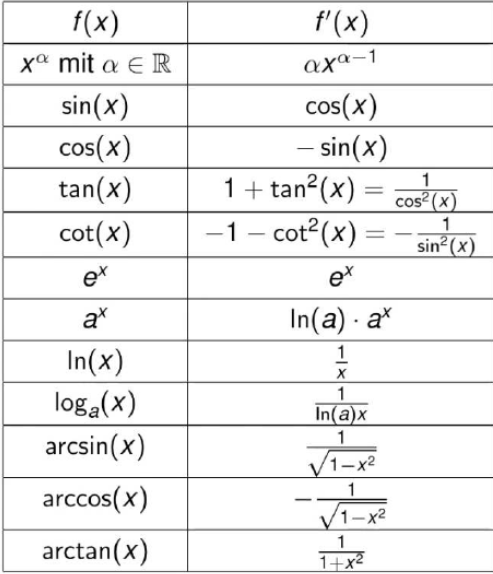
\includegraphics[scale=0.35]{ableitungen.png}
    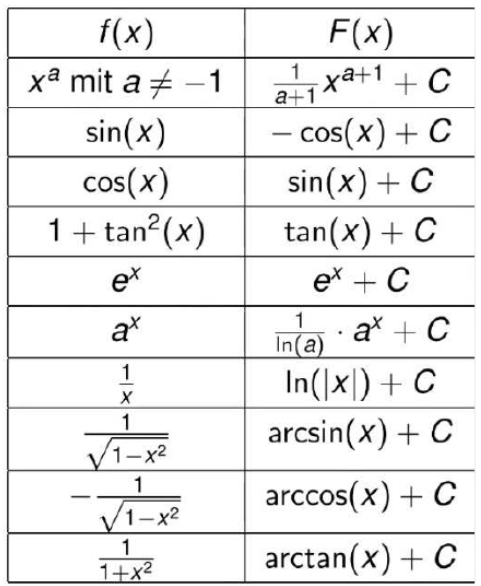
\includegraphics[scale=0.35]{stammfunktionen.png}

    \section{ Ableiten }

    $f(x) = x^n \quad \rightarrow \quad f'(x) = n \cdot x^{n-1}$
    \WhiteSpace
    $f(x) = c \cdot g(x) \quad \rightarrow \quad f'(x) = c \cdot g'(x)$
    \WhiteSpace
    $f(x) = g(x) \cdot h(x) \quad \rightarrow \quad f'(x) = g'(x) \cdot h(x) + g(x) \cdot h'(x)$
    \WhiteSpace
    $f(x) = \frac{g(x)}{h(x)} \quad \rightarrow \quad f'(x)=\frac{h(x) \cdot g'(x) - g(x) \cdot h'(x)}{\left[h(x)\right]^2}$
    \WhiteSpace
    $f(x) = g(h(x)) \quad \rightarrow \quad f'(x) = g'(h(x)) \cdot h'(x)$
    \WhiteSpace

    {Logarithmen:}

    {$f(x) = \ln(x+a) \to f'(x) = \frac{1}{x+a}$}

    {$f(x) = \ln(5x+a) \to f'(x) = \frac{5}{5x+a}$}

    {$f(x) = \ln(-5x+a) \to f'(x) = \frac{-5}{-5x+a}$}
    \WhiteSpace
    \section{ Integrieren }
    \WhiteSpace
    {$$\int x^n dx = \frac{1}{n+1}x^{n+1}+c$$}

    \WhiteSpace
    {$\dfrac{1}{x^5} \rightarrow -\dfrac{1}{4x^4} + C$}
    \WhiteSpace
    \WhiteSpace
    {$\sqrt{x} = x^{\frac{1}{2}} \rightarrow \frac{2}{3}\cdot x^{\frac{3}{2} + C} $}
    \WhiteSpace
    \WhiteSpace
    \vfill\null
    \columnbreak
    \section{Grenzwerte}
    \WhiteSpace
    {Zählergrad $>$ Nennergrad : }

    {\large $ \lim_{n\to \infty} \frac{g(n)}{h(n)} = $ keinen Grenzwert}
    \WhiteSpace

    {Zählergrad $<$ Nennergrad : }

    { \large $ \lim_{n\to \infty} \frac{g(n)}{h(n)} = 0$}
    \WhiteSpace

    {Zählergrad $=$ Nennergrad : }

    {\large $  \lim_{n\to 8} \frac{2n^3+7n...}{5n^3-7n^2...} = \frac{2}{5}$}
    \WhiteSpace

    {$n \to \infty:$}

    {\large  $ \frac{1}{n} = \frac{1}{\infty} = 0$}
    \WhiteSpace




    \subsection{Wahl der Methode}

    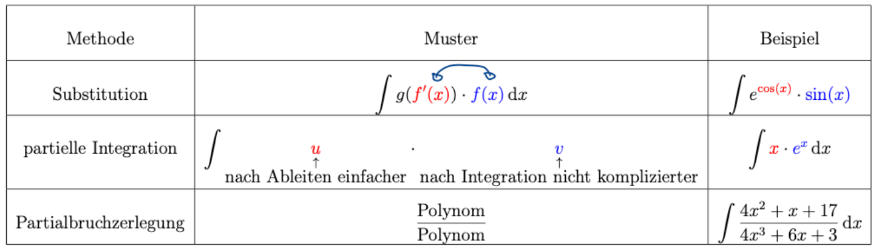
\includegraphics[scale=0.4]{methode.png}

    \subsection{Uneigentliche Integrale}
    { Ein $uneigentliches$ Integral hat die Eigenschaft, dass der Integrationsbereich unendlich gross
        ist oder eine Polstelle enthält.}
    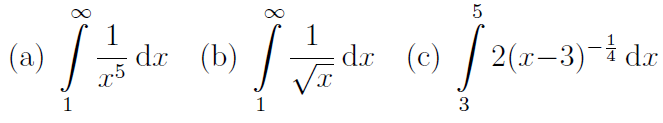
\includegraphics[scale=0.3]{unneigaufgaben.png}

    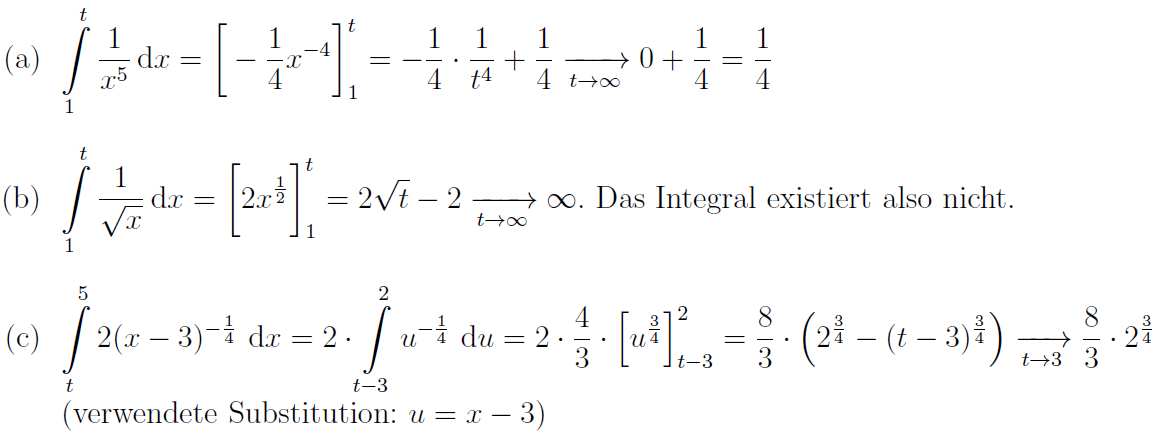
\includegraphics[scale=0.28]{unneigloesng.png}



    \vfill\null
    \columnbreak
    \subsection{Integration durch Substitution}
    {\circled{1} Substitutionsgleichung für $x: u = g(x)$}

    {\circled{2} Substitutionsgleichung für $dx:$}

    $ \frac{du}{dx} = g'(x)_{(Ableitung)} \to dx = \frac{du}{g'(x)}$

    {\circled{3} Integralsubstitution: Einsetzen von $ u $ und $ dx $ aus 1. und 2 in Ursprung}

        {\circled{4} Integration von 3.}

        {\circled{5} Rücksubstitution (nur unbestimmte Integrale)}


    \begin{multicols*}{2}
        {Beispiel:}
        $\int_{}^{}e^{2x} $

        \columnbreak

        {\circled{1} $ u = 2x $}

        {\circled{2} $ dx = \frac{du}{2} $}

        {\circled{3} $ \int_{}{}e^u \cdot  \frac{du}{2} $}

    \end{multicols*}

    {\circled{4} $ \int_{}{}e^u \cdot  \frac{1}{2}du = \frac{1}{2} \cdot  \int_{}{}e^u du \rightarrow \frac{1}{2} e^u + C   $}


    {\circled{5} $\frac{1}{2} e^u + C \rightarrow \frac{1}{2} e^{2x} + C$ }




    \subsection{Partielle Integration}
    {\large $$u(x)\cdot v(x) - \int_{}^{}u'(x) \cdot v(x) \hspace{2px}  dx$$}

    \begin{multicols*}{2}
        {Beispiel:}
        \[ \int_{}{}x\cdot e^x\]

        $$ \int_{}{}x\cdot e^x = x\cdot e^x -  \int_{}{}\cdot e^x dx = x\cdot e^x - e^x + C $$
        \columnbreak

        {$u(x)=x$; $v'(x)=e^x$}

        {$u'(x)=1$; $v(x)=e^x$}

    \end{multicols*}


    \vfill\null
    \columnbreak


    \subsection{Integration durch Partialbruchzerlegung}
    {\circled{1}    Polynomdivision (falls Funktion unecht gebrochen!): Zählergrad  $>$ Nennergrad }



    {\circled{2} \textbf{Nullstellen} des Nenners bestimmen (raaten, 2Klammeransatz, Horner, lösen)}

    {\circled{3} Jeder Nullstelle ihren Partialbruch zuordnen:}

    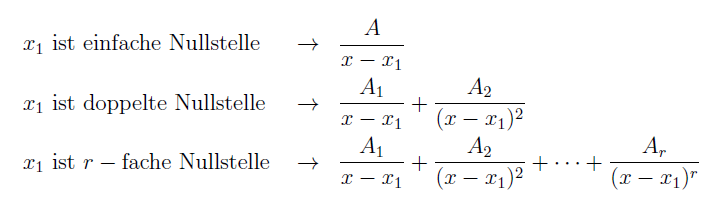
\includegraphics[scale=0.5]{partialbruch.png}
    {\circled{4} Ansatz zur Partialbruchzerlegung aufstellen $\rightarrow$ $f(x)$ wird mit der Summe aller Partialbrüche gleichgesetzt}

    {\circled{5} Bestimmung der Konstanten $A,A_1,A_2,...,A_r$}
    \begin{enumerate}
        \itemsep0em
        \item Brüche gleichnamig machen
        \item Einsetzen von x-Werten (Nullstellen) $\rightarrow$ LGS
        \item LGS lösen $\rightarrow$ man erhält die Konstanten $A,A_1,B,...$
    \end{enumerate}


    {\circled{6} Integration der Partialbrüche}

    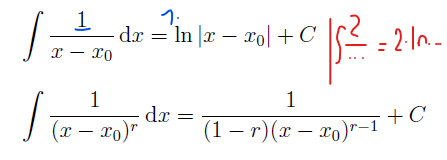
\includegraphics[scale=0.5]{integr_partial.png}

    {\textbf{Beispiel}: \large $\int_{}^{}\frac{5x+11}{x^2+3x-10}dx $ }
    \begin{enumerate}
        \itemsep-0.3em
        \item ist echt gebrochen: ok
        \item Nullstellen Nenner: $ (x-2)(x+5) \Rightarrow x_0 = 2; x_1 = -5$
        \item $ \frac{A}{x-2}+\frac{B}{x+5}$
        \item \large $\int_{}^{}\frac{5x+11}{x^2+3x-10}dx  = \frac{A}{x-2}+\frac{B}{x+5}$
        \item     \begin{enumerate}
                  \itemsep-0.3em
                  \item    $\int_{}^{}\frac{5x+11}{x^2+3x-10}dx = \frac{A(x+5)+B(x-2)}{(x-2) +(x+5) }$
                  \item \small $5x + 11 = A(x+5)+B(x-2) $
                  \item  {\small einsetzen:  $ x = 2 \rightarrow A=3; $ $ x = -5 \rightarrow B=2; $}
              \end{enumerate}
        \item  $\int_{}^{}\frac{5x+11}{x^2+3x-10}dx =\int_{}^{}\frac{3}{x-2}+\frac{2}{x+5}dx  \newline = 3\cdot ln(|x-2|) + 2\cdot ln(|x+5|) + C $
    \end{enumerate}

    \vfill\null
    \newpage
    \section{Differentialgleichungen (DGL)}
    \subsection{Begriffe}
    {\textbf{Ordnung:} Ordnung = höchste Ableitung in der DGL}
    {\textbf{Linearität:} Funktion und Ableitung sind linear $\rightarrow x^1$ }

    \subsection{Separierbare Differentialgleichungen}
    {Eine Differentialgleichung 1. Ordnung heisst separierbar wenn:}
    $$ y' = f(x)\cdot g(y)$$

    {How To:}

    \circled{1}$y' = \frac{dy}{dx} = f(x)\cdot g(y) $

    \circled{2} {Trennung der Variablen:} $\frac{dy}{g(y)} = f(x)\cdot dx$

    \circled{3} {Integration auf beiden Seiten der Gleichung (if possible):} $$\int_{}^{}{\frac{dy}{g(y)}=\int_{}^{}f(x)dx}$$
    \circled{4} {Auflösen nach y (falls möglich!)}

    \begin{multicols}{2}
        {Beispiel:}

        $$y' = y^2 = sin(x)$$

        \circled{1} $y' = \frac{dy}{dx}=\frac{sin(x)}{y^2}$

        \circled{2} $y^2\cdot dy = sin(x)\cdot dx $
        \columnbreak

        \circled{3}

        \circled{4}

    \end{multicols}



    \subsection{Autonome Differentialgleichungen}
    {Definition: $y' = f(y)$}
    {$\Rightarrow$ Diese Differentialgleichungen sind separierbar!}
    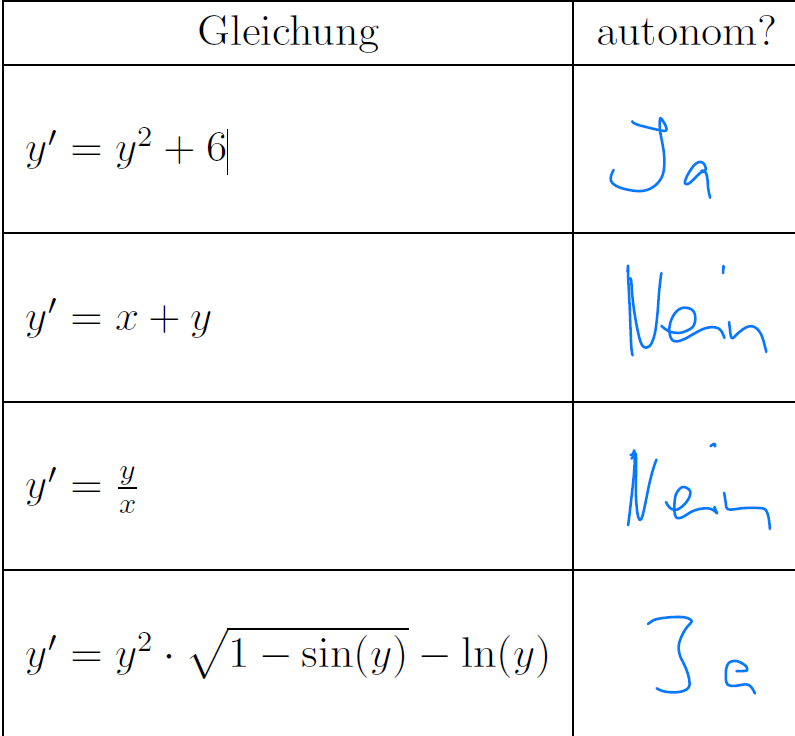
\includegraphics[scale=0.2]{autonom.png}
    \vfill\null
    \columnbreak
    \subsection{ Lineare Differentialgleichungen}
    {\large Form: $y' + f(x) \cdot y = g(x)$}

    {$g(x) \rightarrow$ Störglied / Störfunktion}

    { "linear" $\rightarrow$ $y$ und $y'$ in der ersten Potenz}

    { $homogen \rightarrow$ wenn das Störglied  $g(x)=0$}

    { ansonsten $\rightarrow$ $inhomogen$}

    \subsection{ Variation der Konstanten für lineare Differentialgleichungen}

    \circled{1}{ Bestimmung von $f(x)$ und $g(x)$ basierend auf: }

    {       $y' + f(x) \cdot y = g(x)$}

    \circled{2}{ Bestimmung der Stammfunktion $F(x)$ von $f(x)$}

    \circled{3}{ Einsetzen in die Formel \large $y_0 = K(x) \cdot e^{-F(x)}$}

    \circled{4} {$K$ berechnen: \large $K(x) = \int g(x) \cdot e^{F(x)} dx $}


    \circled{5}{ $K$ in Ansatz aus \circled{3} einsetzten $\rightarrow$ allgemeine Lösung}



    {Beispiel:}

    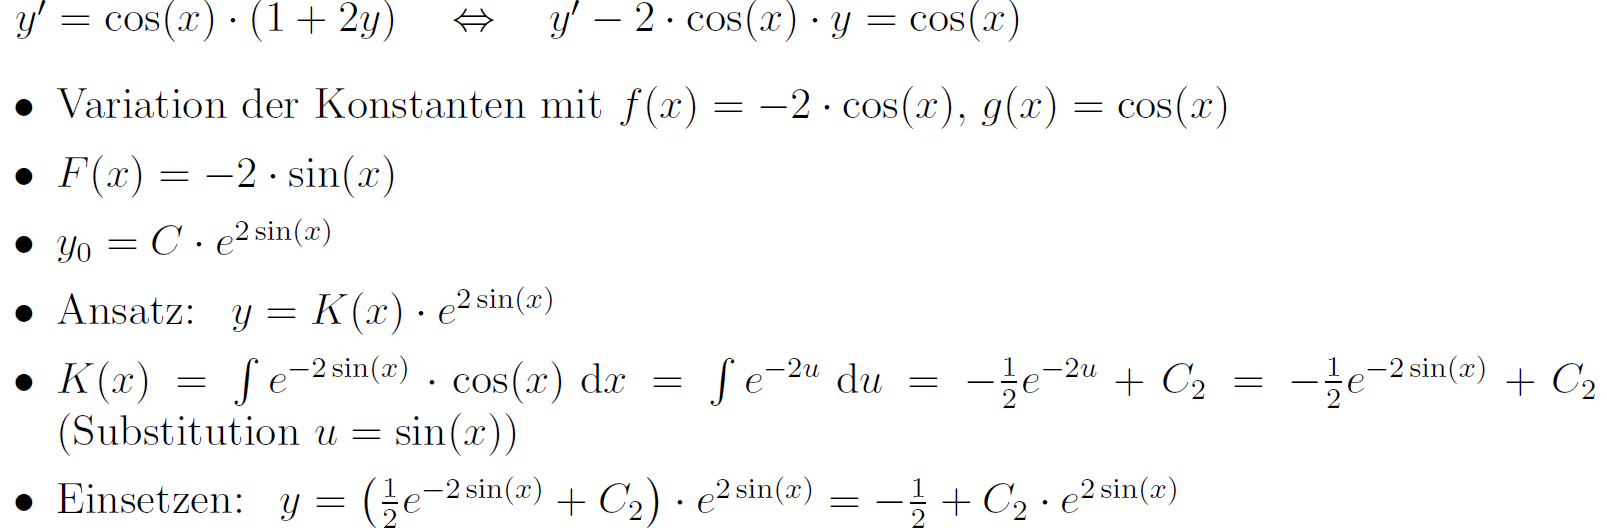
\includegraphics[scale=0.22]{variation_der_k_bsp.png}


    \subsection{ Richtungsfelder}

    \circled{1}{ DGL in die Form $y'=f(x,y)$ bringen.}

    \circled{2}{ Bereich wählen, welcher zur veranschaulichung optimal ist. (Bspw: $-2$ - $2$)}

    \circled{2}{ Nun setzt man in diesem Bereich $x$ und $y$ Werte ein und Liest die resultierende $Steigung$ ab. Diese Steigung wird dann am Punkt eingetragen.}

    \subsection{ Eulerschritte}

    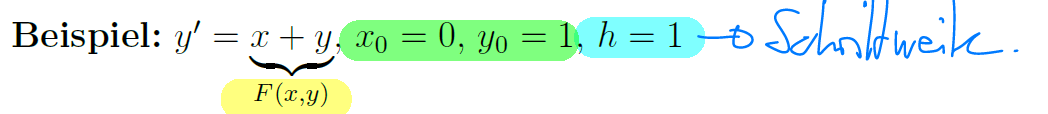
\includegraphics[scale=0.3]{euler.png}

    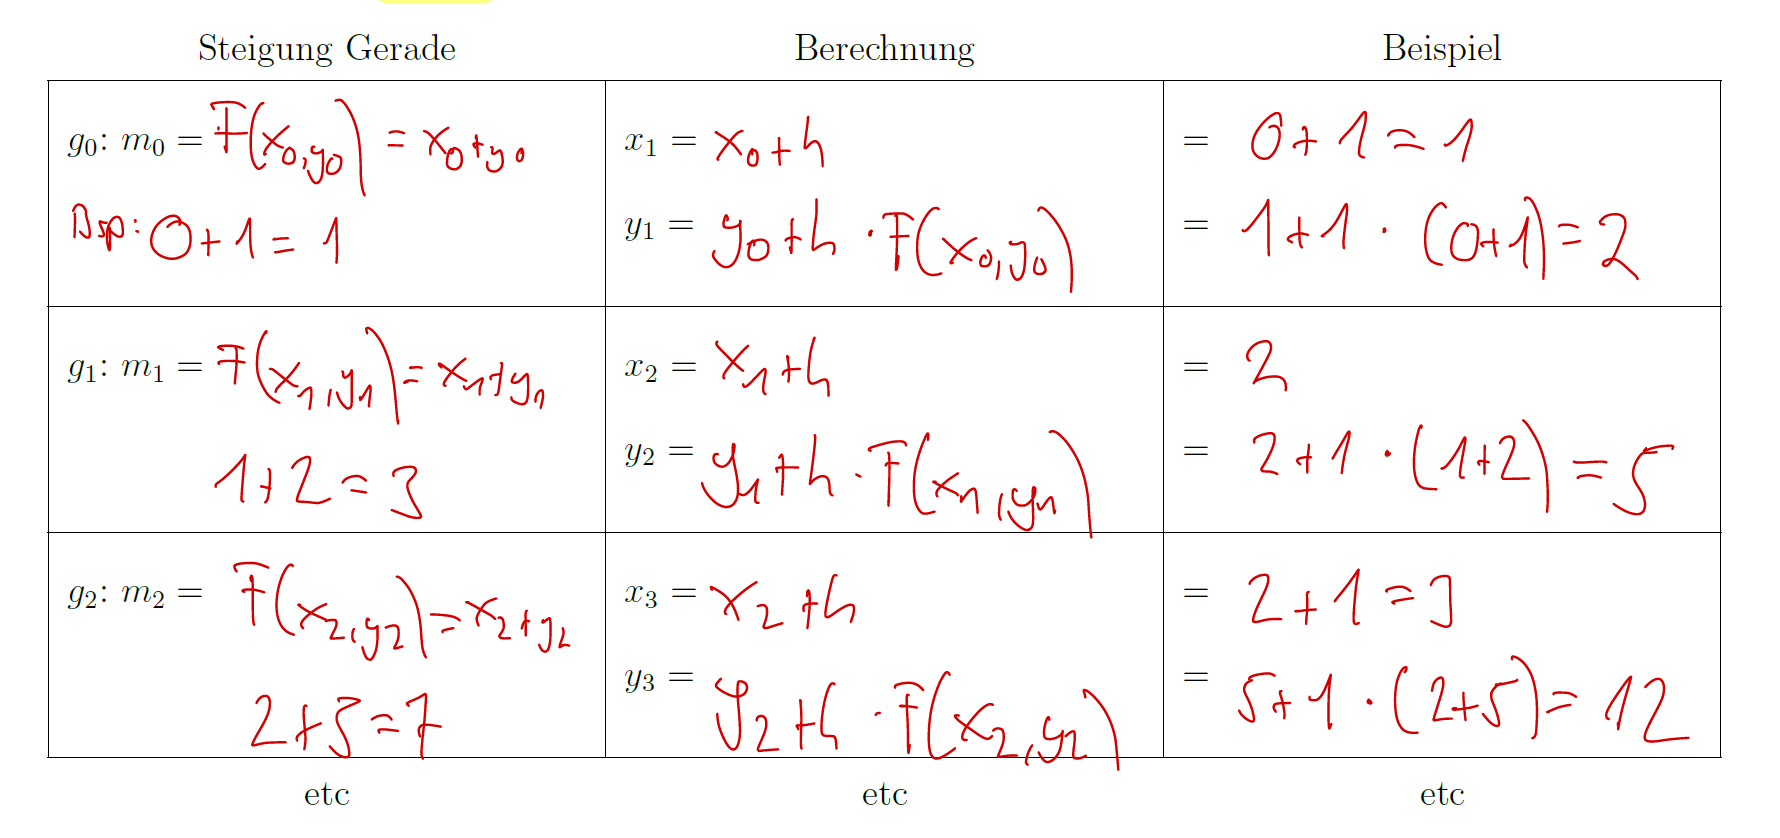
\includegraphics[scale=0.22]{euler_2.png}

    \vfill\null
    \columnbreak

    \section{Anwendungen der Intergralrechnung}
    \subsection{Rotation um die x-Achse}

    \begin{multicols}{2}

        {$$V = \pi \cdot \int_{a}^{b}(f(x))^2dx$$}

        \columnbreak
        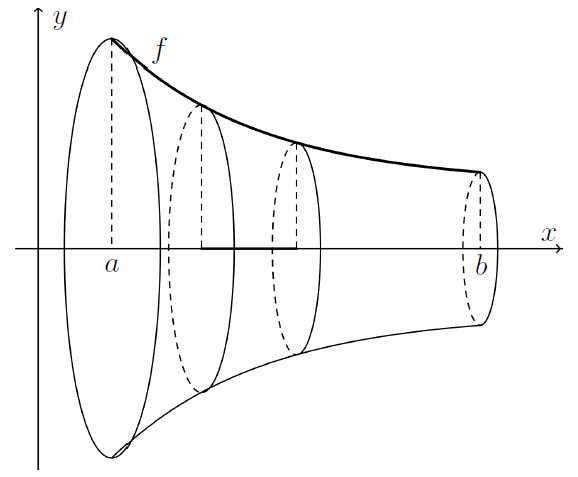
\includegraphics[scale=0.3]{rotationskoerper.png}
    \end{multicols}


    \subsection{Rotation um die y-Achse}

    \begin{multicols}{2}

        {$$V = \pi \cdot \int_{c}^{d}(g(y))^2dy$$}

        $\rightarrow$ $g(y)$ die nach $x$ aufgelöste Funktionsgleichung.

        \columnbreak
        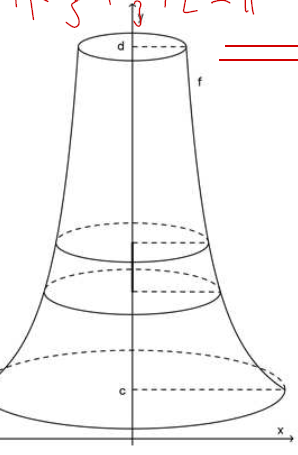
\includegraphics[scale=0.35]{rotationskoerper_y.png}
    \end{multicols}



    \subsection{Bogenlänge einer ebenen Kurve (Graph)}

    \begin{multicols}{2}

        {$$s = \int_{a}^{b}\sqrt{1+(y')^2}dx$$}

        \columnbreak
        \includegraphics[scale=0.35]{bogenlänge.png}


    \end{multicols}

    \subsection{Mantelfläche eines Rotationskörpers}

    {$$M = 2\pi \int_{a}^{b} y \cdot \sqrt{1+(y')^2}dx$$}
    \vfill\null
    \columnbreak
    \subsection{Schwerpunkt Fläche zwischen zwei Kurven}

    \begin{multicols}{2}

        {$$x_s =\frac{1}{A}\cdot \int_{a}^{b}x \cdot(f_o(x)-f_u(x))dx$$}

        {$$y_s =\frac{1}{2A}\cdot \int_{a}^{b}(f_o^2(x)-f_u^2(x))dx$$}

        \columnbreak
        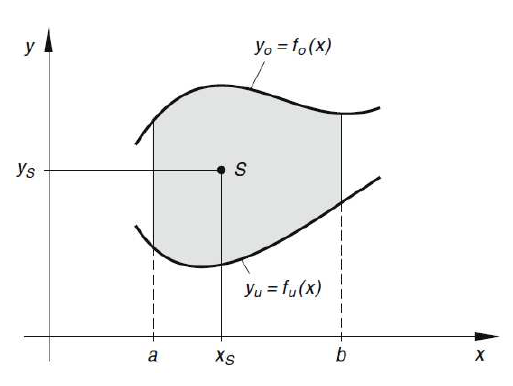
\includegraphics[scale=0.35]{schwerpunkt.png}


    \end{multicols}


    \subsection{Schwerpunkt eines Rotationskörpers}

    \begin{multicols}{2}

        {$$x_s =\frac{1}{V}\cdot \int_{a}^{b}x \cdot f^2(x)dx$$}

        {$$y_s = 0 , z_s = 0$$}

        \columnbreak
        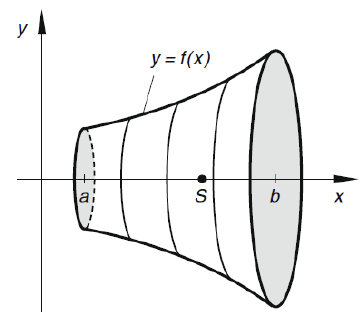
\includegraphics[scale=0.35]{schwerpunkt_rotationskoerper.png}

    \end{multicols}

    \vfill\null
    \newpage
    \section{Taylor-Reihen}
    \subsection{Definition}
    {Eine Funktion $f(x)$ entspricht einer Taylorreihe mit unendlich vielen Gliedern. Die Stelle $x_0$ ist die Entwicklungsstelle. Die Entwicklungsstelle ist die Stelle, in deren Umgebung uns das Verhalten der Funktion interessiert.}
    \WhiteSpace
    \subsection{Verfahren / Formel}

    \begin{multicols*}{2}

        $$t_f = \sum_{k = 0}^{ \infty }\frac{f^n(x_0)}{k!}\cdot(x-x_0)^k$$

        \columnbreak
        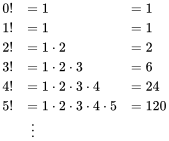
\includegraphics[scale=0.5]{fak.png}

    \end{multicols*}
    {Grad: $anzahl$ Ableitungen / Schritte}

    {\circled{1} Ableitungen bilden (Grad)}
    \WhiteSpace
    {\circled{2} $x_0$ in Ableitungen einsetzen}
    \WhiteSpace
    {\circled{3} Ableitungen in Formel einsetzen}
    \WhiteSpace
    {\circled{4} ausrechnen/kürzen/vereinfachen}
    \WhiteSpace
    {Beispiel:}

    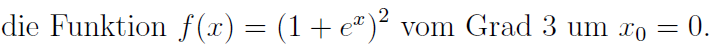
\includegraphics[scale=0.35]{taylor_example.png}

    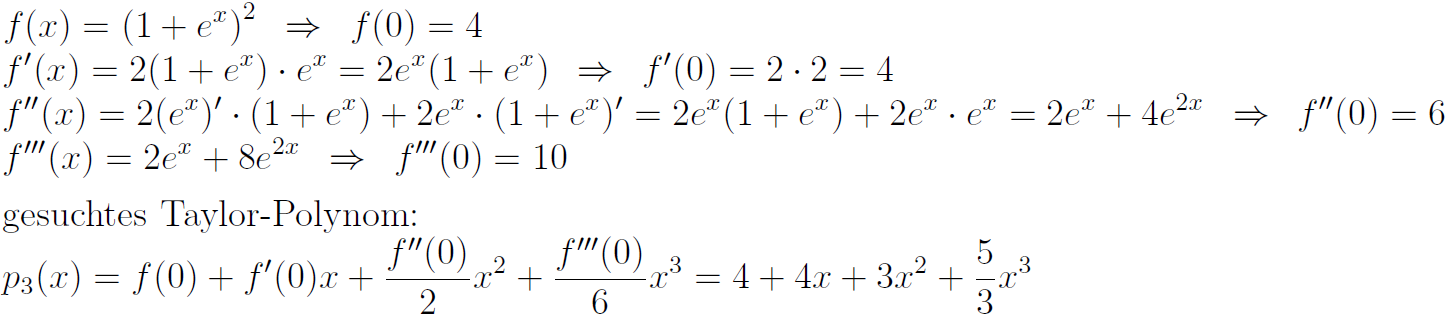
\includegraphics[scale=0.25]{taylor_example_sol.png}
    \vfill\null
    \columnbreak
    \subsection{Bekannte Taylorreihen}

    { 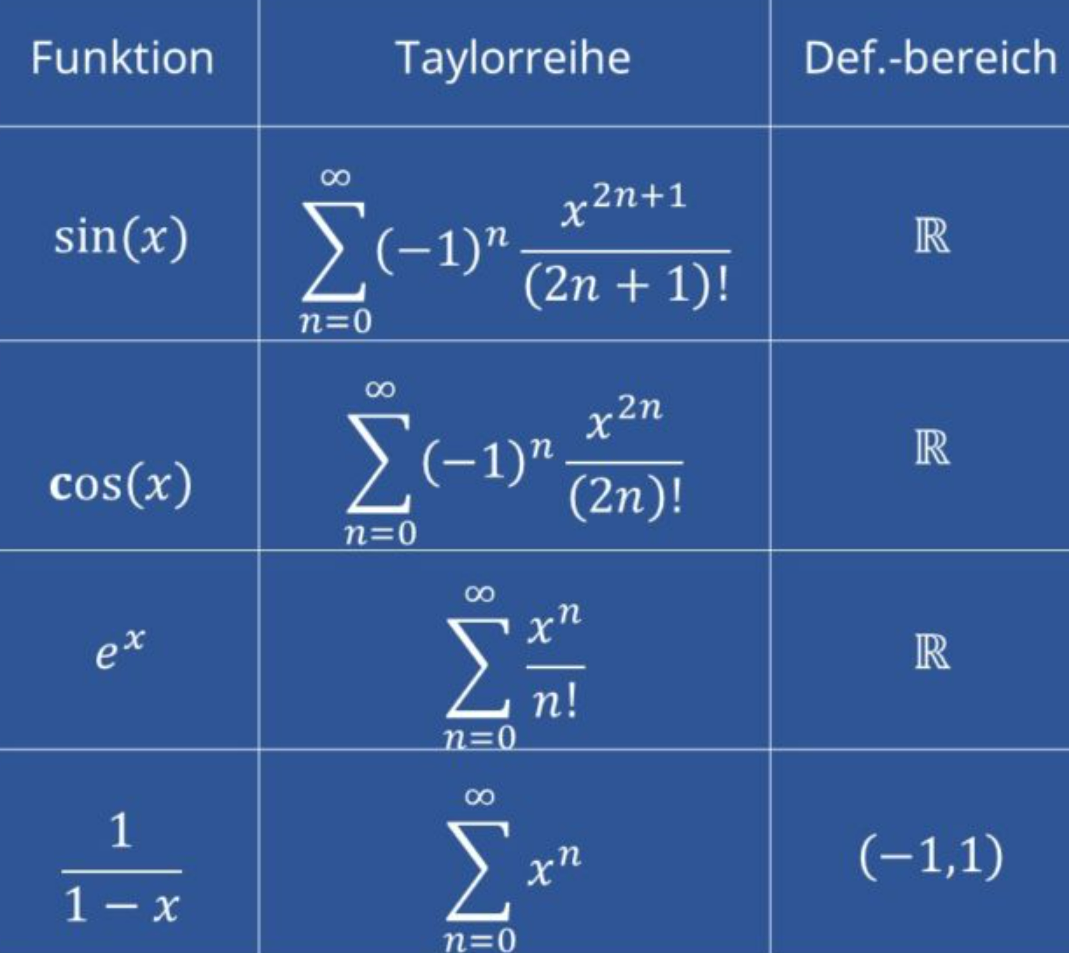
\includegraphics[scale=0.5]{taylor_overvieqw.png} }

    { 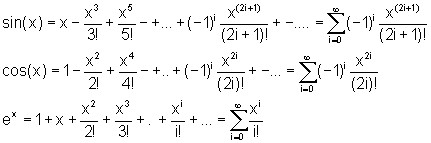
\includegraphics[scale=2.5]{taylor7.jpg} }

    \subsection{Mitternacht}
    { 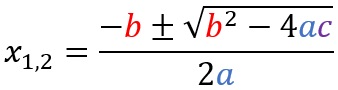
\includegraphics[scale=0.5]{1556295318.jpg} }

    \vfill\null
    \columnbreak


    \section{Konvergenzen}
    \subsection{Konvergenzradius bei Taylor}

    $$P(x) = \sum_{k = 0}^{ \infty }a_k\cdot(x-x_0)^k$$

    {$$r:= \lim_{k \to \infty } |\frac{a_k}{a_{k+1}}| $$}

    {$r:$ Konvergenzradius}

    {\textbf{Berechnung:}}

    {$$\sum^{\infty}_{k=1}{\frac{1}{k^2}\cdot x^k}$$}

    {In $r$ Formel einsetzen $\to$ (ohne den $x$ Teil)}

    {$$ \lim_{k \to \infty} \frac{\frac{1}{k^2}}{\frac{1}{(k+1)^2}} = \frac{(k+1)^2}{k^2} = (\frac{k+1}{k})^2 = (\frac{k+1}{k}) \cdot (\frac{k+1}{k})  $$}

    {$$\implies k \to \infty \implies (\frac{\infty+1}{\infty}) \cdot (\frac{\infty+1}{\infty}) = 1 \cdot 1 = 1  =r$$}

    \textbf{Bestimmung Intervall konvergiert:}

    {$\to$ Einsetzen von $x_0$ und $r$ in folgende Definition:}

    {($x_0$) aus $P(x)$ ablesen. Wenn nicht vorhanden: unendlichen Konvergenzradius und konvergiert für ganz $R$ }


    {alle $x \in (x_0 -r,x_0 + r)$zum Konvergenzbereich gehören }



    {alle $x \in (-\infty,x_0 - r)$ NICHT zum Konvergenzbereich gehören }


    \subsection{Regel von Bernoulli-Hopital}


    $$ \lim_{x \to x_0} \frac{g(x)}{h(x)} = \lim_{x \to x_0} \frac{g'(x)}{h'(x)}$$

    {\circled{1} Zählerfunktion $g(x)$ und Nennerfunktion $f(x)$ getrennt voneinander ableiten}
    \WhiteSpace
    {\circled{2} Grenzewert von $\frac{g'(x)}{h'(x)}$ brechnen}
    \WhiteSpace

    {\textbf{BEM:} Die Regel von L'HOSPITAL kann auch mehrfach hintereinander angewendet werden.}
    {\small(Wenn Lösung nacht 1x ableiten nicht ersichtlich)}
    \mbox{}

\end{multicols*}

\end{document}
